\textbf{La base de datos Animales con Atributos (Animals with Attributes) contiene información sobre 50 animales. Para cada uno, se tienen 85 caracterÍsticas de valor real que capturan varias propiedades del animal: dónde vive, qué come, etc. Esta es claramente una aplicación en la que esperamos que la agrupación descubra “grupos naturales” en los datos.}

\begin{itemize}
    \item Usa ISOMAP, LLE, T-SNE y SOM's para encontrar visualizaciones informativas de los datos.
    \item Aplique el algoritmo de Clustering Jerarquico usando las funciones linkage: single, complete,
          ward.
\end{itemize}
Muestre los dendogramas correspondientes y responda las siguientes preguntas basado en los resultados obtenidos

\begin{enumerate}
    \item Hasta qué punto tienen éxito estos algoritmos en esta tarea?
    \item Son los grupos en su mayoría razonables?
    \item Podemos, en general, esperar que la agrupación capte perfectamente lo que queremos?
    \item Para cual(es) funcion(es) de linkage estaría satisfecho con el agrupamiento? Comente su respuesta.
\end{enumerate}

El resultado del análisis debe ser un pequeño reporte con textos e imágenes integrados.

\section*{Visualizaciones informativas}

A partir de los datos contenidos en el archivo \file{predicate-matrix-continuous.txt} se realizaron los procesos de Isomap, LLE, T-SNE y SOM para obtener visualizaciones de la distribución de los datos.

\subsection*{Isomap}

En la figura \ref{fig:isomap} se visualizan los resultados que obtuvo al aplicar isomap. En estos resultados se visualiza que existe una diferencia entre ciertos grupos de animales. Por ejemplo en la parte superior derecha se realizo la agrupación del gorilla y el chimpancé. En la parte inferior derecha animales como la morca y la orca también se encuentran cercanos. En la parte central se puede ver que realizo la agrupación de animales domesticos junto a animales que pertenecen a la misma familia.

\begin{figure}[H]
    \centering
    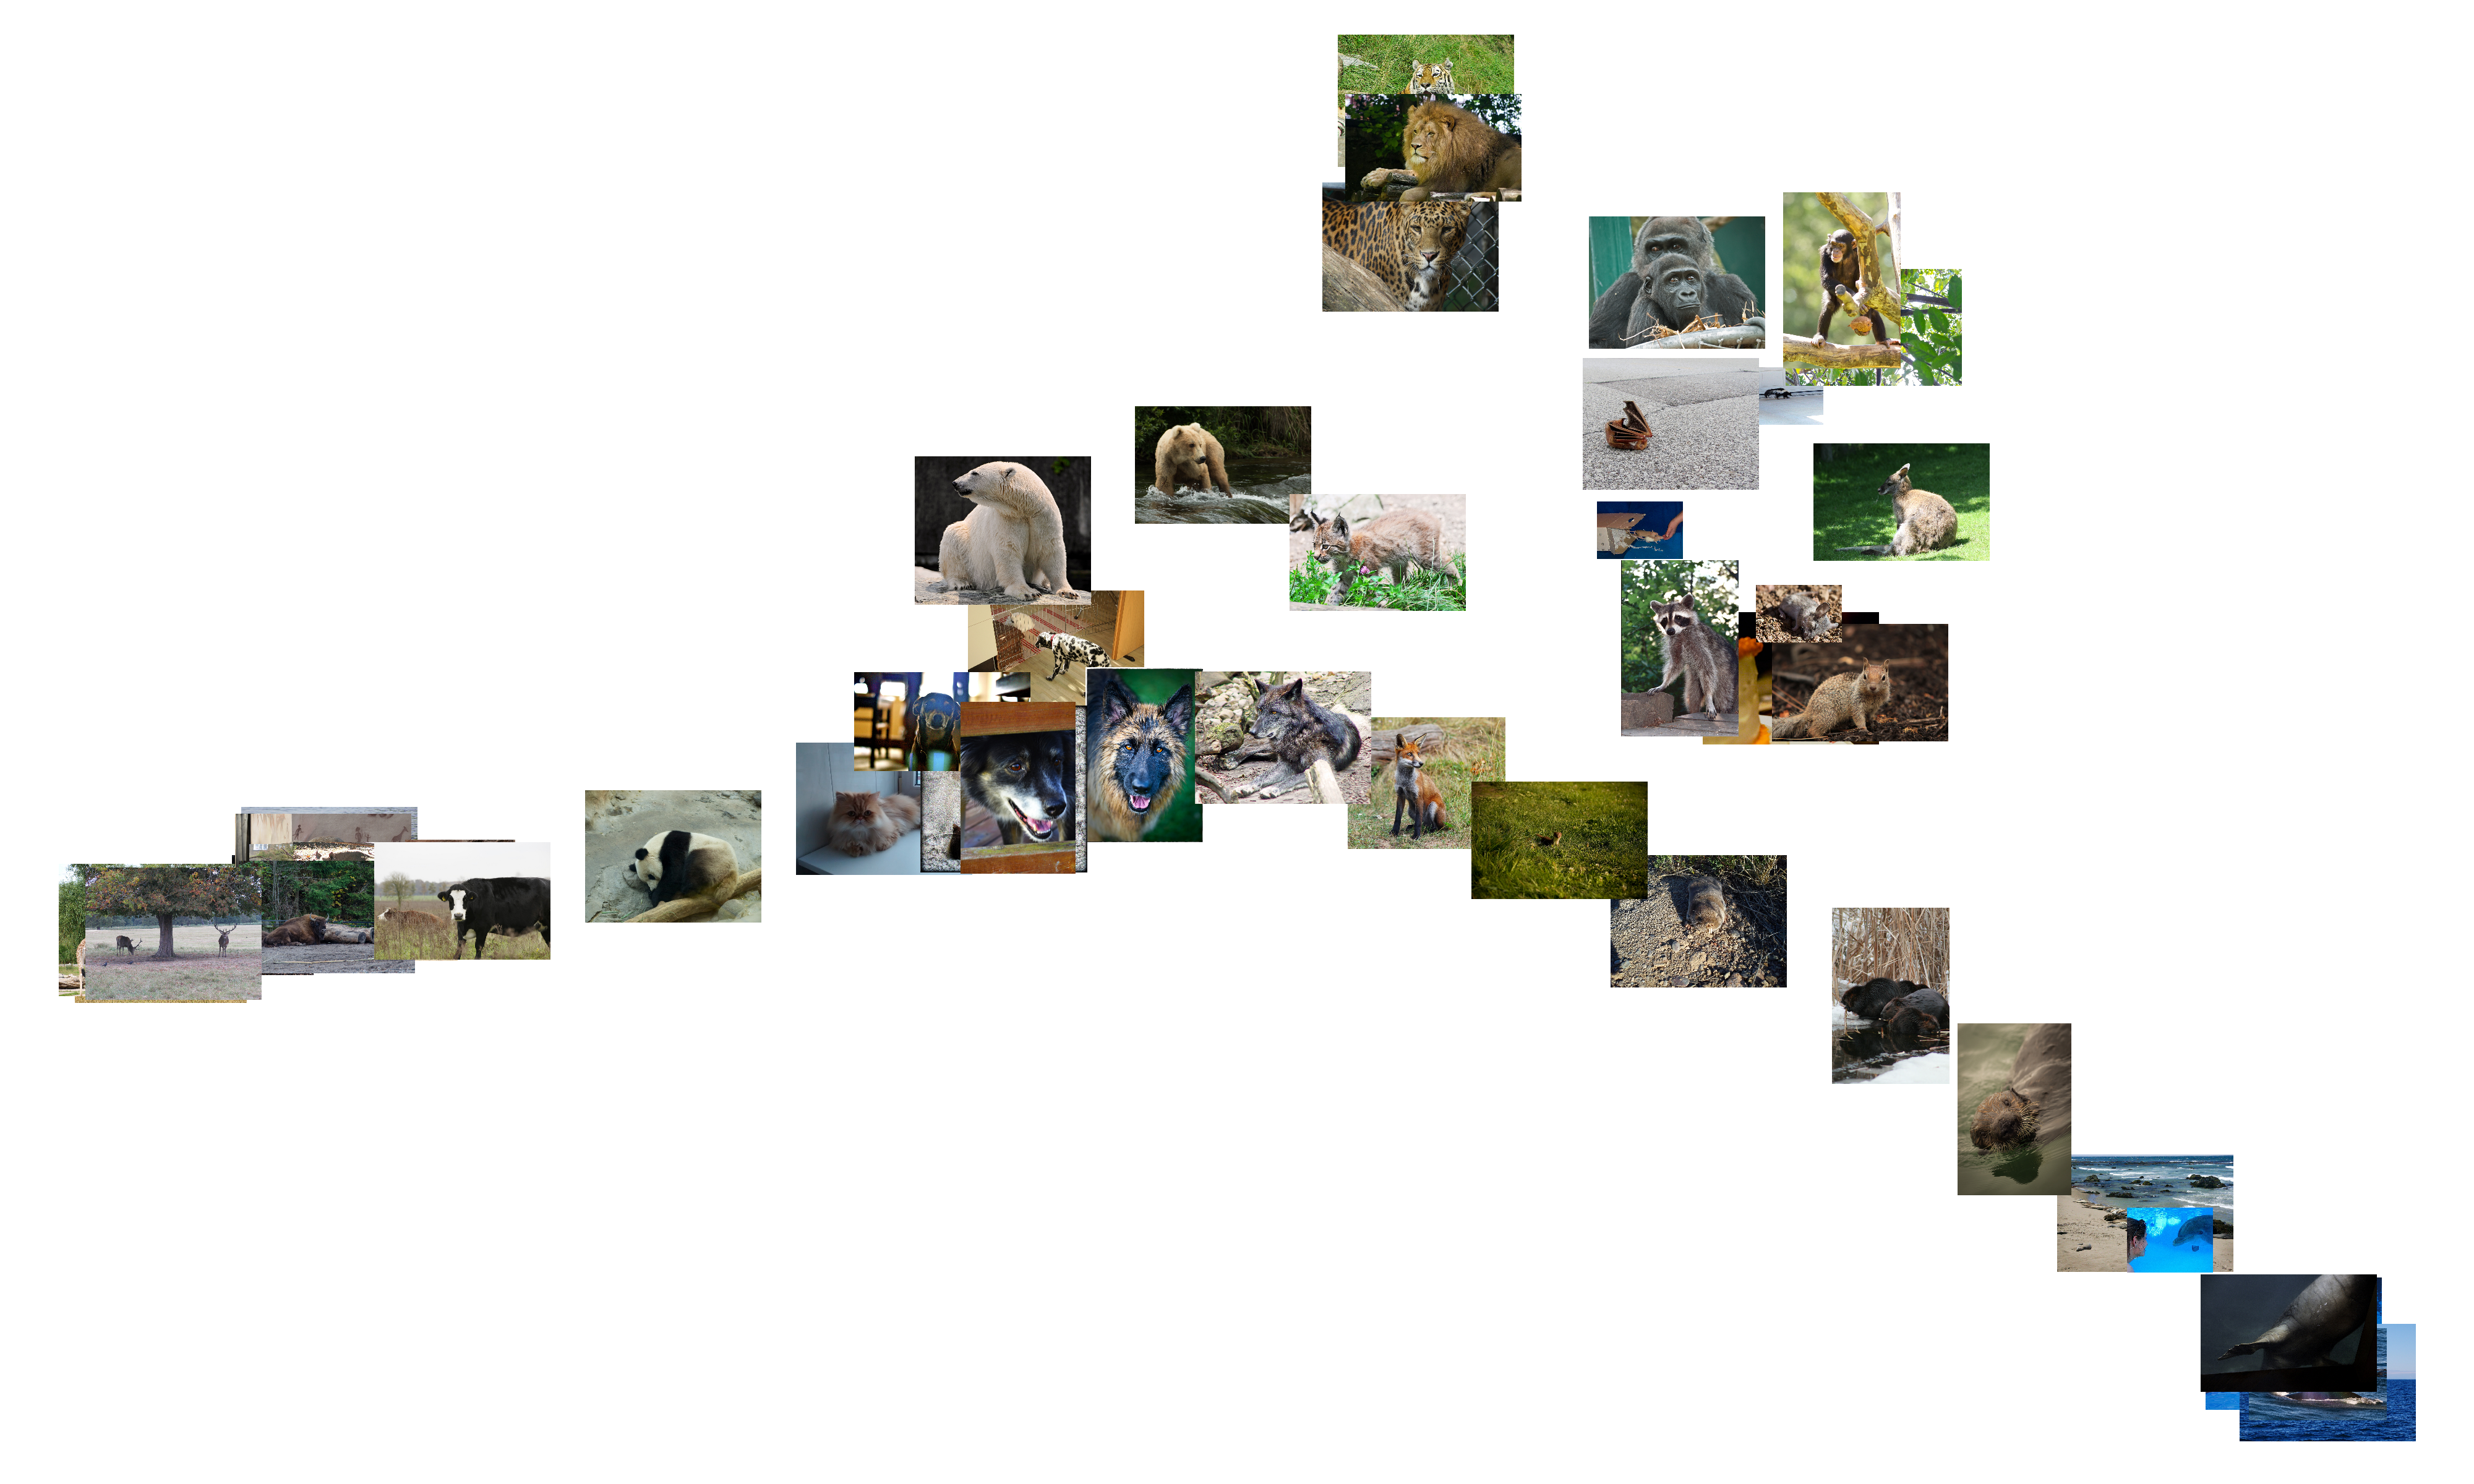
\includegraphics[width=12cm,height=8cm]{Graphics/Isomap.png}
    \caption{Resultados de aplica el isomap a los datos contenidos en el archivo \file{predicate-matrix-continuous.txt}.}
    \label{fig:isomap}
\end{figure}

\subsection*{LLE}

En la figura \ref{fig:LLE} se visualiza el resultado que se obtuvo al aplicar LLE a los datos. A diferencia del método de isomap, LLE realizo una mayor distinción entre animales maritimos y terrestres. Realizando un grupo de animales pertenecientes a las granjas y primates. En otros casos no llego a realizar la distinción entre animales domesticos.

\begin{figure}[H]
    \centering
    \includegraphics[height=8cm,width=12cm]{Graphics/LLE.png}
    \caption{Resultados de aplica LLE a los datos contenidos en el archivo \file{predicate-matrix-continuous.txt}.}
    \label{fig:LLE}
\end{figure}

\section*{T-SNE}

En la figura \ref{fig:tsne} se observan los resultados que se obtuvo al aplicar T-SNE a los datos. A diferencia de los métodos anteriores, en T-SNE no se logra visualizar agrupamientos de animales con gran distinción. Se observa que los animales acuaticos ocupan la parte de la derecha. Los primates se encuentran en la parte superior y animales salvajes como el tigre y león se encuentran en la parte de la izquierda. Revisando más a detalle se observa que la mayoria de los animales domensticos se encuentran en la parte central.

\begin{figure}[H]
    \centering
    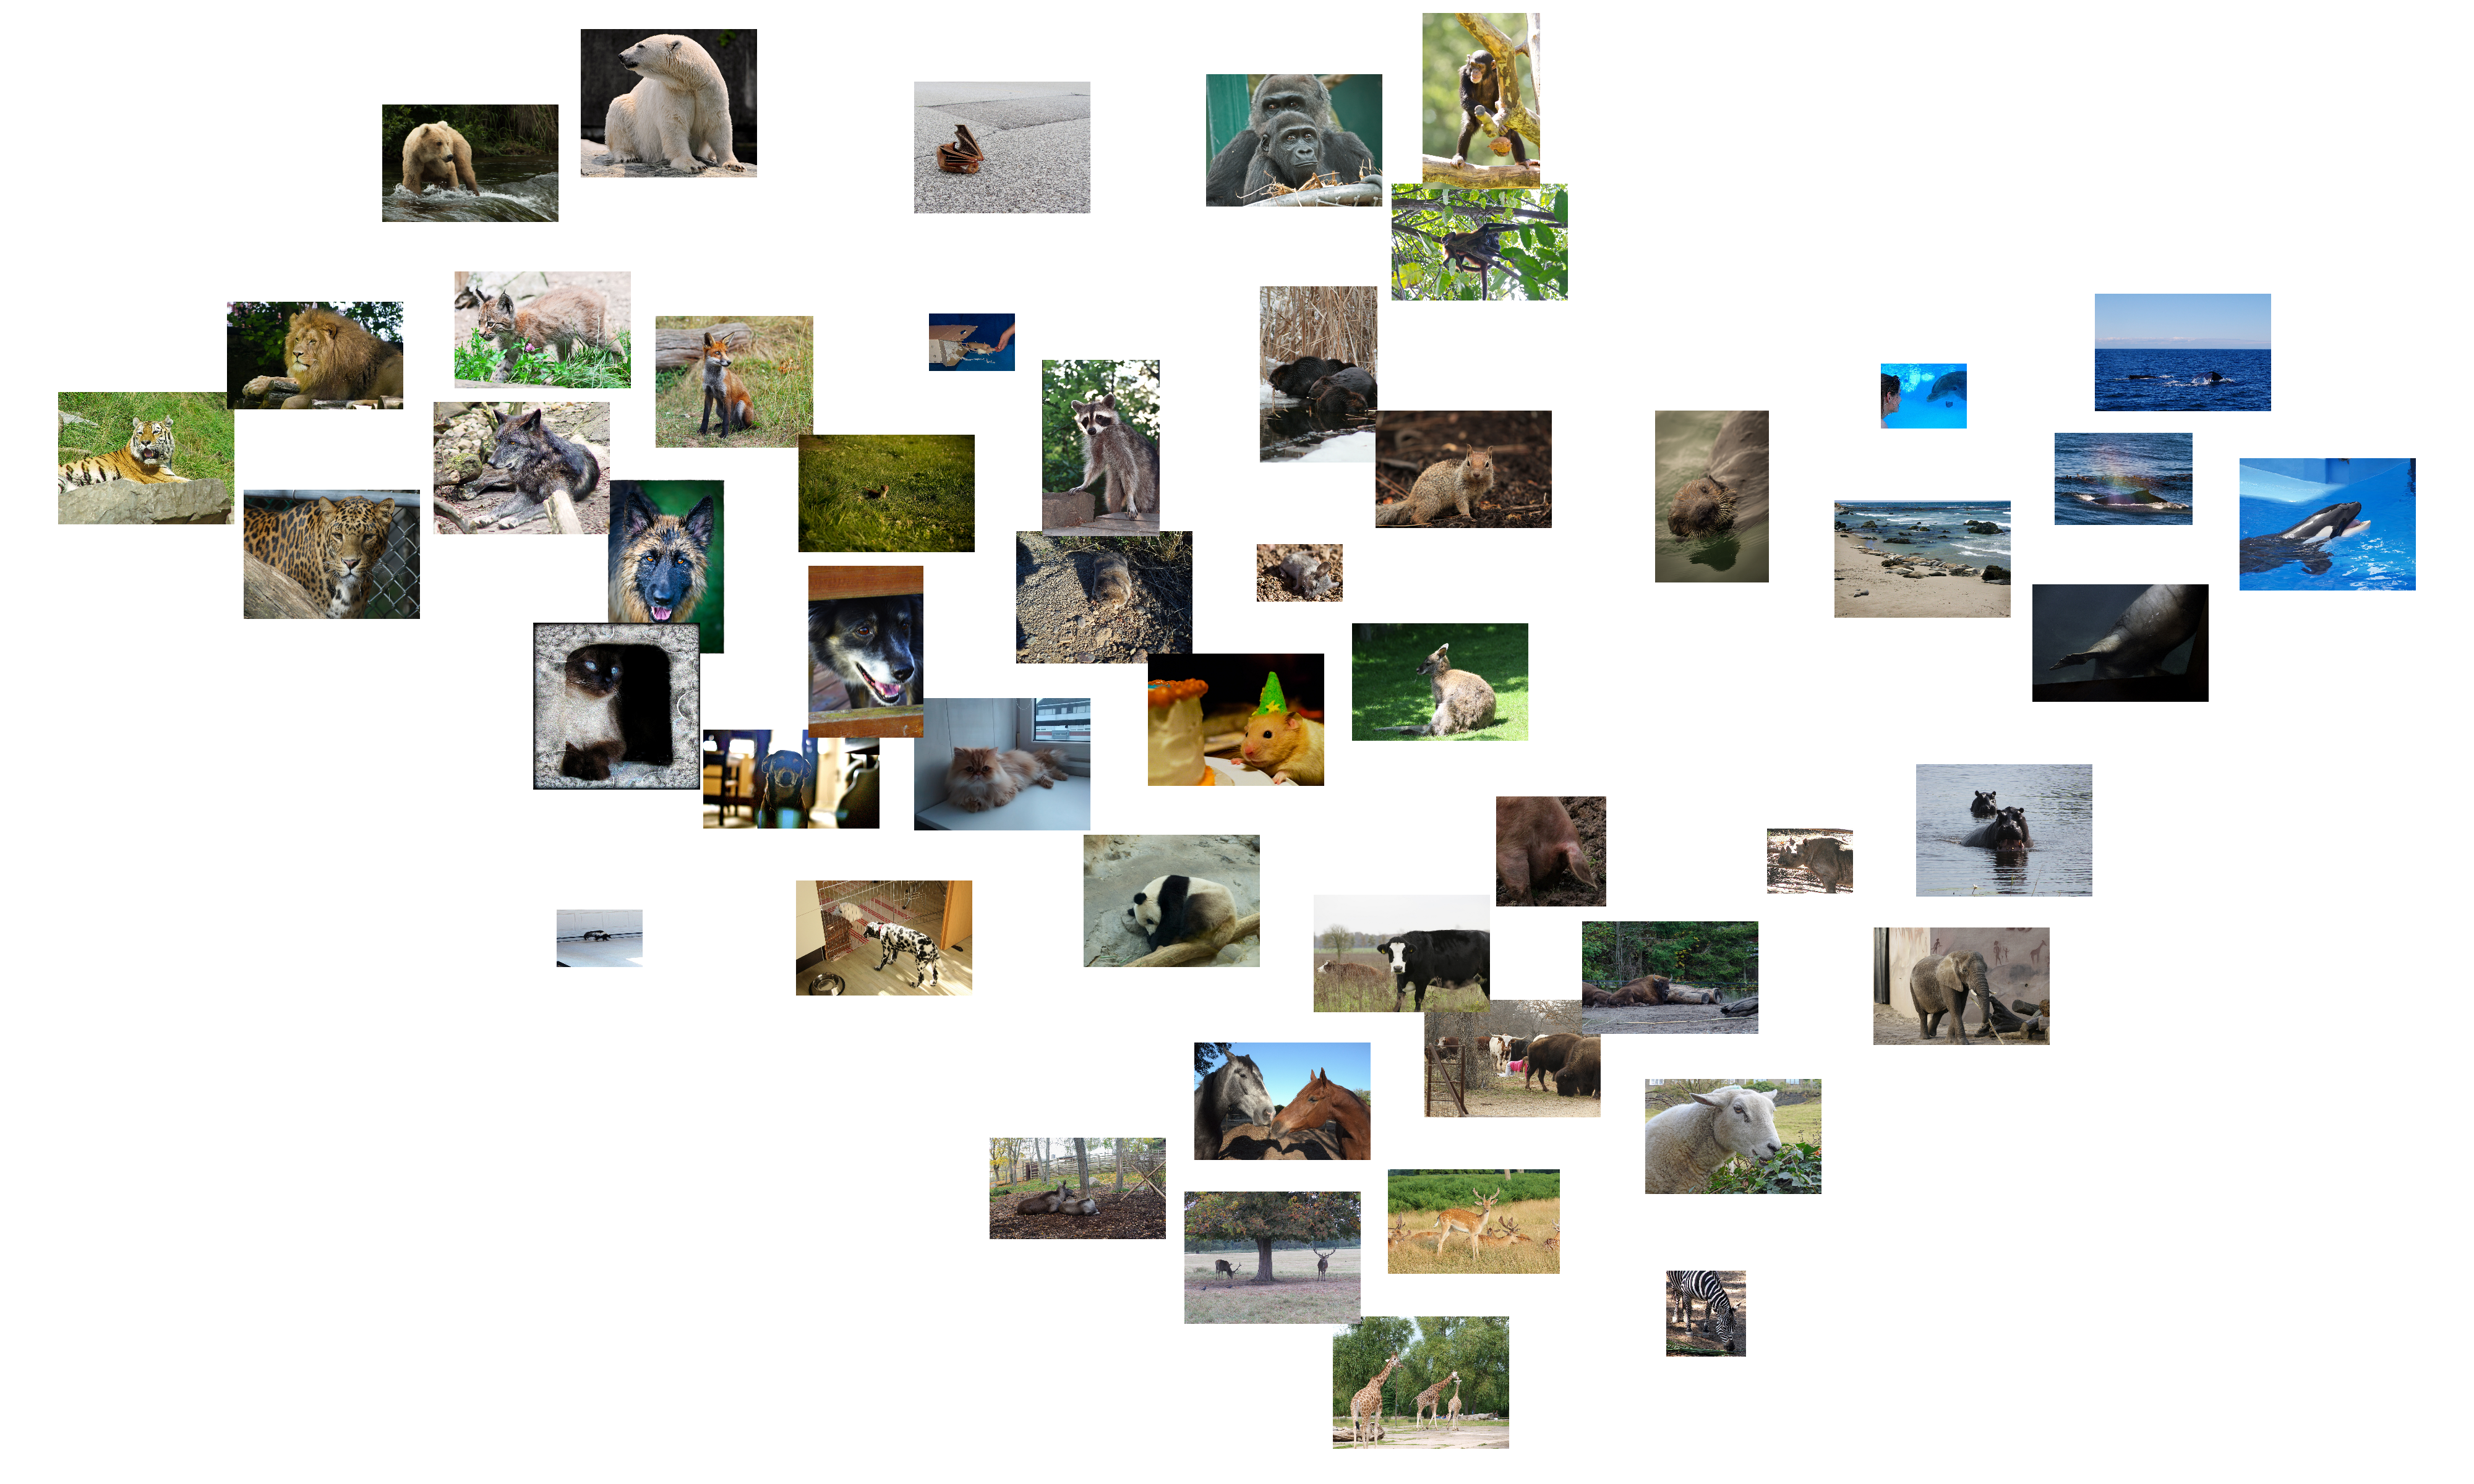
\includegraphics[height=8cm,width=12cm]{Graphics/TSNE.png}
    \caption{Resultados de aplica LLE a los datos contenidos en el archivo \file{predicate-matrix-continuous.txt}.}
    \label{fig:tsne}
\end{figure}

\section*{SOM}

Los métodos anteriores realizan una reducción de dimensionalidad en los datos. Esto funciona para reconocer si existen grupos en los datos. En la figura \ref{fig:som} se representan los grupos encontrados por SOM en la parte izquierda y en la parte derecha la posición de cada animal en cada reducción de orden antes calculada. Con SOM se logra delimitar de una mejor manera los resultados obtenidos en cada reducción de orden identificando a cada animal en una clase.

\begin{figure}[H]
    \centering
    \begin{subfigure}{17cm}
        \centering
        \includegraphics[width=8cm]{Graphics/SOM_isomap.png}
        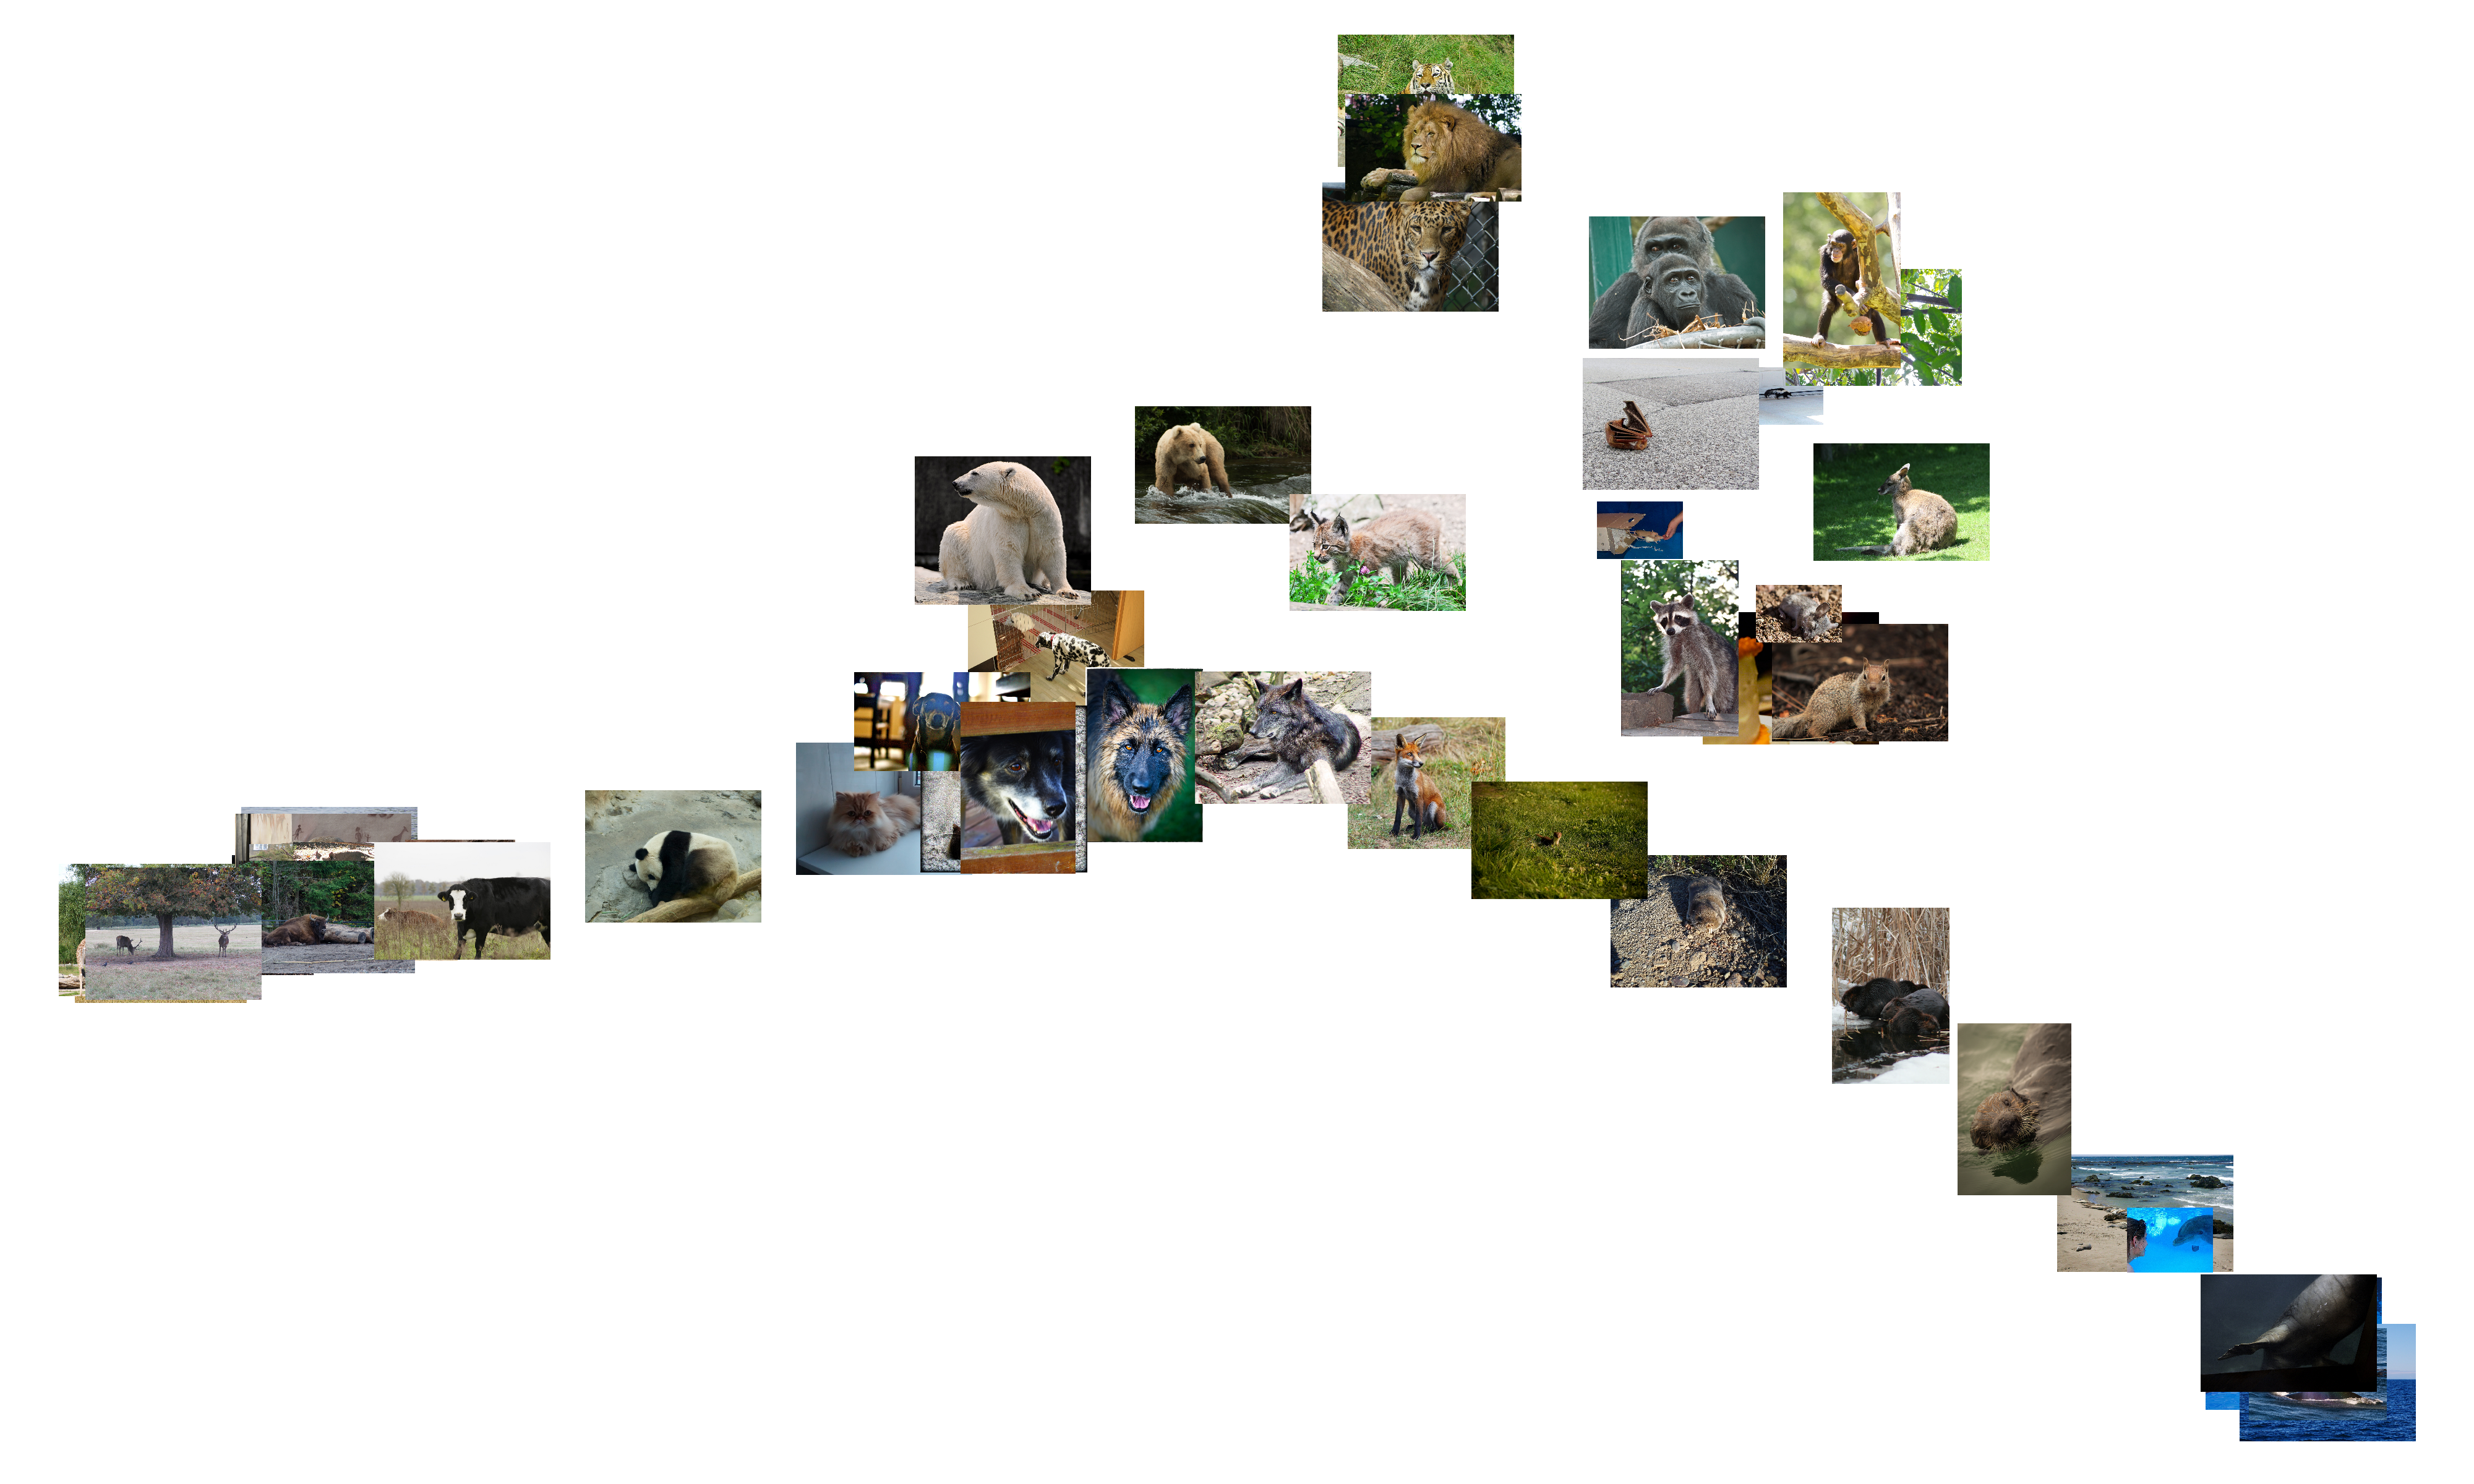
\includegraphics[width=8cm]{Graphics/Isomap.png}
        \caption{Isomap}
    \end{subfigure}
    \begin{subfigure}{17cm}
        \centering
        \includegraphics[width=8cm]{Graphics/SOM_LLE.png}
        \includegraphics[width=8cm]{Graphics/LLE.png}
        \caption{LLE}
    \end{subfigure}
    \begin{subfigure}{17cm}
        \centering
        \includegraphics[width=8cm]{Graphics/SOM_TSNE.png}
        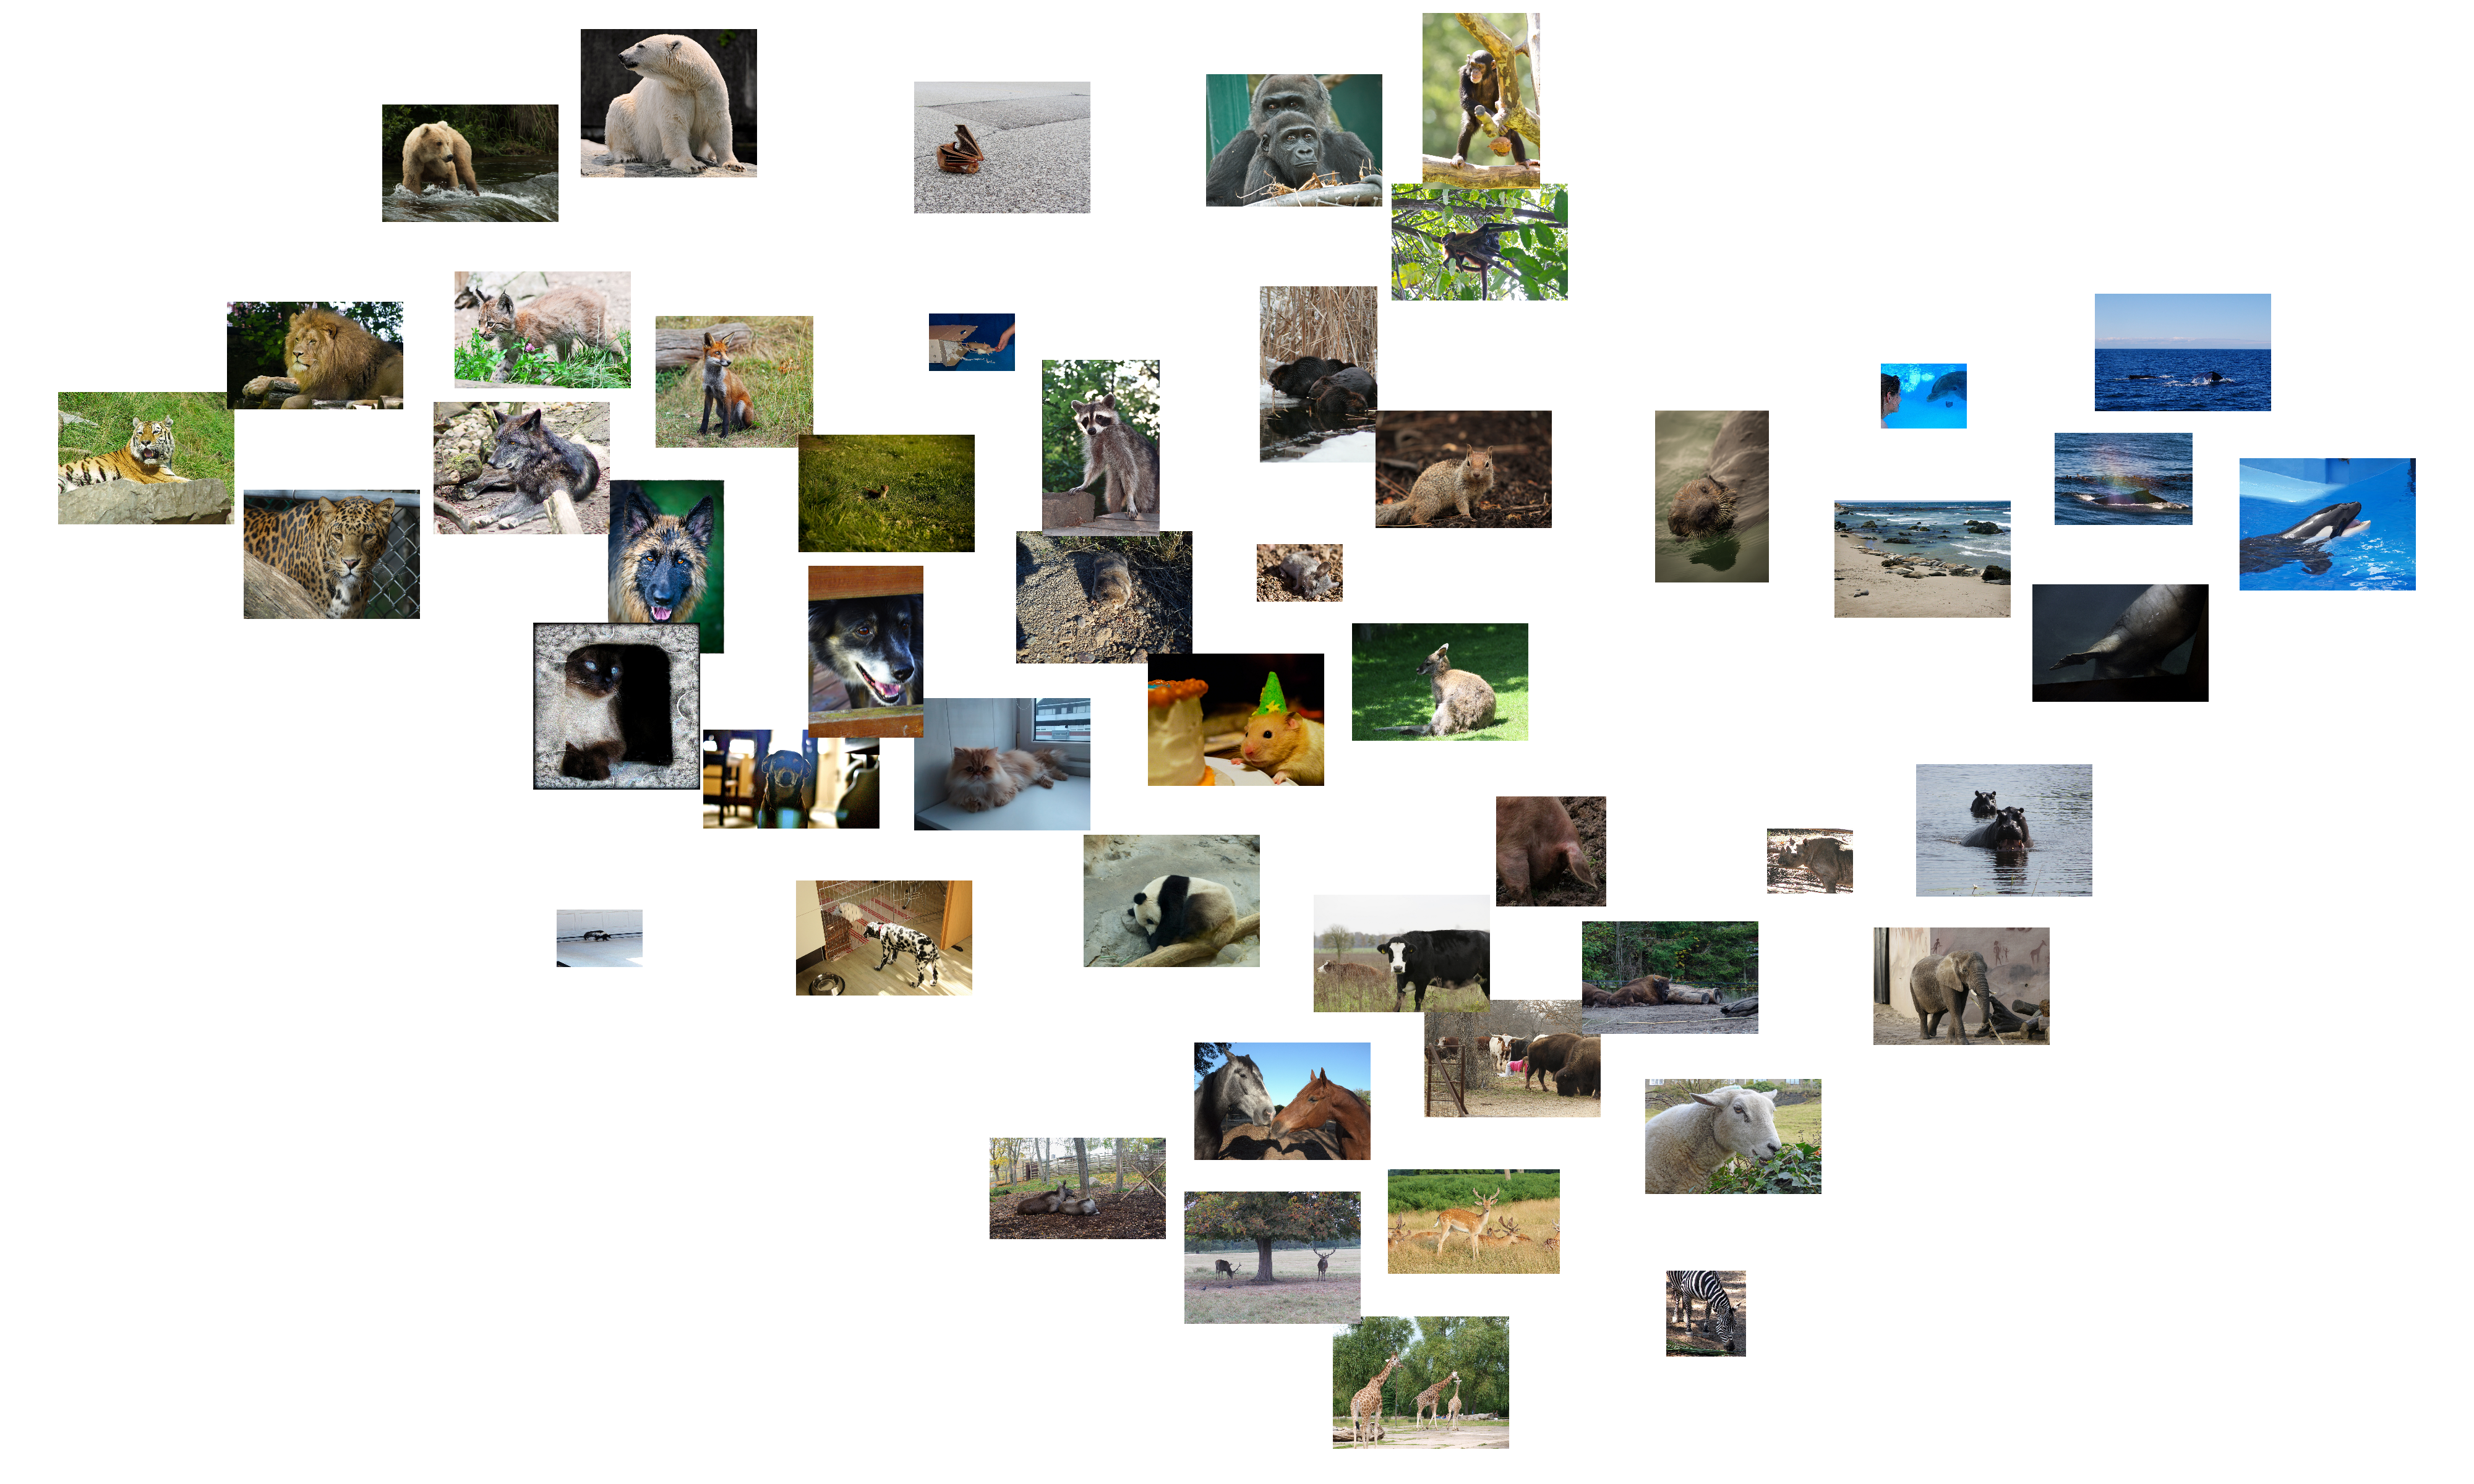
\includegraphics[width=8cm]{Graphics/TSNE.png}
        \caption{T-SNE}
    \end{subfigure}
    \caption{Resultados de apliar SOM a el conjunto de datos con cada reducción de dimensión}
    \label{fig:som}
\end{figure}

